\documentclass{article}
\usepackage[english]{babel}
\usepackage{hyperref}
\usepackage{tcolorbox}
\usepackage{graphicx}
\usepackage{amsmath}
\graphicspath{ {images/} }


\title{Tutorial manual: constraint-based modeling for systems medicine }
\author{Thierry D.G.A. Mondeel \and Stefania Astrologo \and Hans V. Westerhoff}

\begin{document}
\maketitle

\tableofcontents

\section*{The platform: SageMath}

We will use the online SageMath platform for this tutorial.

\begin{quote}
SageMath is a free open-source mathematics software system licensed under the GPL. It builds on top of many existing open-source packages: NumPy, SciPy, matplotlib, Sympy, Maxima, GAP, FLINT, R and many more. Access their combined power through a common, Python-based language or directly via interfaces or wrappers.
Mission: Creating a viable free open source alternative to Magma, Maple, Mathematica and Matlab.
\end{quote}

\begin{tcolorbox}[width=\textwidth,colback={yellow},title={ASSIGNMENT},coltitle=white]

It is best to follow this tutorial in groups of two or three students. This will reduce the server load and allow you to discuss together. Please form a group now if you have not yet.
\end{tcolorbox}

\begin{tcolorbox}[width=\textwidth,colback={yellow},title={ASSIGNMENT},coltitle=white]

Go to \url{https://cloud.sagemath.com/} and register for an account. Then tell the tutorial supervisors the user name of your account so that we can add you to the tutorial project on SageMath.
\end{tcolorbox}

\subsection*{A note about doing this on your own laptop}
The software required to do constraint-based modeling is not quickly installed. For this reason we utilize the online SageMath platform which already has the required software installed.
If you would like to do similar work offline on your own laptop you will require the following things:
\begin{itemize}
\item A python distribution with Jupyter notebook installed: we recommend the anaconda scientific python distribution. See: \url{https://www.continuum.io/downloads}.
\item Cameo and Cobrapy will require you to have glpk. See: \url{https://www.gnu.org/software/glpk/}.
\item When you have Anaconda installed you can install Cobrapy and Cameo on top of it. By running the following command (cameo will automatically also install escher and cobrapy)
\begin{verbatim}
pip install cameo
\end{verbatim}

For more details see \url{https://github.com/biosustain/cameo}.

\end{itemize}

If you're interested you may try this after today's tutorial. 

Another very good online alternative developed at the VU by Brett Olivier is \url{F-A-M-E.org} which gives you an environment to perform constraint-based modeling without having to code anything.

\section*{Setting up your own workspace}
\addcontentsline{toc}{section}{Getting Started: setting up your own workspace}

Once the tutorial supervisor has added you to the project: the "systems me\-di\-cine tutorial" project will appear in your list of projects on SageMath.

\textbf{WATCH OUT:} The files in this project are editable by you. We do not want you to edit the original files so you will have to create your own \emph{copy} of them. The sequence of steps to do this is outlined below.

\begin{tcolorbox}[width=\textwidth,colback={yellow},title={ASSIGNMENT},coltitle=white]

\begin{itemize}
\item Navigate to the main folder of this project. If you are anywhere in the Sagemath website you can get there through the "Projects" button and then selecting the project for this tutorial.
\item From the main folder of the project navigate to the "Students" subfolder.
\item Click "Create" at the top of the screen.
\item Type in your name (this will be the name of your own personal folder) and then click "Folder"
\item You will now automatically end up in your own folder, however it will be empty. Lets fix that!
\item Navigate back to the main folder by clicking "Parent Directory" twice.
\item Check the box next to the "tutorial\_files" folder.
\item Then click copy and select your personal folder in the drop down menu "Destination" in the top-right of the screen.
\item Now navigate to your personal folder again. 
\end{itemize}
\end{tcolorbox}

You should now have a personal folder with the tutorial files in them. You can safely edit these files to your heart's content!

If anything goes really wrong, you can always copy the original tutorial files back to your personal folder again.

\section*{Overview and introduction}
\addcontentsline{toc}{section}{Overview and introduction}

Now that you have your own space to work we can start the tutorial. The aim of this tutorial is to introduce you to constraint-based modeling and the applications of the human metabolic reconstruction RECON2 \cite{Thiele2013}. 

\textbf{Note of warning:} this is the first time we give this tutorial on this platform so please forgive us for any mistakes/shortcomings. The website might be a bit slow at times, be patient please.

There are various software packages that enable the user to perform con\-straint-based~modeling. We will use the Python based: Cameo \url{https://github.com/biosustain/cameo} and Cobrapy \cite{Ebrahim2013}. This requires you to know at least some basics of python which is what we will start the tutorial with. If you already have experience with Python feel free to skim (not skip) the first part. Even if you already have some experience there may be some tips and tricks in the first part that will come in handy later.

After the Python introduction we will introduce the Cameo package and how to do computational analysis on the human metabolic reconstruction with it. Specifically, we will investigate tyrosine and phenylalanine metabolism and biomarker predictions for inborn errors of metabolism like phenylketonuria.

Happy computing!

\section{Introduction to Python \& Jupyter}

To do our computational analysis on the human metabolic reconstruction we will make use of the Python programming language.

Some exerpts from the wiki page on Python \url{https://en.wikipedia.org/wiki/Python_(programming_language)}
\begin{quote}
Python is a widely used high-level, general-purpose, interpreted, dynamic programming language. Its design philosophy emphasizes code readability, and its syntax allows programmers to express concepts in fewer lines of code than would be possible in languages such as C++ or Java. The language provides constructs intended to enable clear programs on both a small and large scale.

Python was conceived in the late 1980s, and its implementation began in December 1989 by Guido van Rossum at Centrum Wiskunde \& Informatica (CWI) in the Netherlands as a successor to the ABC language (itself inspired by SETL) capable of exception handling and interfacing with the operating system Amoeba. Van Rossum is Python's principal author, and his continuing central role in deciding the direction of Python is reflected in the title given to him by the Python community, benevolent dictator for life (BDFL).

The core philosophy of the language is summarized by the document The Zen of Python (PEP 20), which includes aphorisms such as:\\
- Beautiful is better than ugly \\
- Explicit is better than implicit\\
- Simple is better than complex\\
- Complex is better than complicated\\
- Readability counts
\end{quote}

We will write simple python code to do constraint-based modeling on the human metabolic map using so-called Jupyter notebooks:
\begin{quote}
Notebook documents (or “notebooks”, all lower case) are documents produced by the Jupyter Notebook App which contain both computer code (e.g. python) and rich text elements (paragraph, equations, figures, links, etc...). Notebook documents are both human-readable documents containing the analysis description and the results (figures, tables, etc..) as well as executable documents which can be run to perform data analysis.
\end{quote}

We have generated several such notebooks for you. These contain ever more complex commands and analysis and build on one another. Each notebook contains some examples of how to do specific things and one or more small questions and assignments.

\subsection*{Getting to know the Jupyter notebook}

\begin{tcolorbox}[width=\textwidth,colback={yellow},title={ASSIGNMENT},coltitle=white]

All Jupyter notebooks for this tutorial are located in the "tutorial\_files" folder within your personal folder.
We will go through them in their numbered order, so your first Jupyter notebook is "0\_running\_code\_in\_notebook.ipynb" etc.

Open the first file and go through the various commands within in. It will introduce you to the basics of the notebook. Make sure you interact with the document. Execute code cells manually, don't just look at it, and do the assignments.

\textbf{This part should not take more than 15 minutes.}
\end{tcolorbox}

\subsection*{Python essentials}
Now that we know our way around the Jupyter notebook it's time to become a bit more familiar with Python itself so that you are able to to do computational analysis later on.

\begin{tcolorbox}[width=\textwidth,colback={yellow},title={ASSIGNMENT},coltitle=white]

Go through tutorial 1: "1\_introduction\_to\_python.ipynb" until the section "Functions". The material from functions onward is not needed to understand the rest of the tutorial. If you have time to spare later on, you can go back to this tutorial.

Again, if you are familiar with Python already, feel free to skim this tutorial.

\textbf{This tutorial should take you about 30 min. to go through.}
\end{tcolorbox}

\section{Introduction to CAMEO}
Now that we understand some basic Python syntax we can get into the specific python packages that allow us to do constraint-based modeling analyses on the human metabolic map. The following tutorial will introduce the Cameo package.

\begin{quote}
\url{http://cameo.bio/} (Developed at the Novo Nordisk Foundation Center for Biosustainability)

Cameo is a high-level python library developed to aid the strain design process in metabolic engineering projects. The library provides a modular framework of simulation methods, strain design methods, access to models, that targets developers that want custom analysis workflows.
\end{quote}

The cameo website showcases some basic Jupyter notebooks on how the use the package.

\begin{tcolorbox}[width=\textwidth,colback={yellow},title={ASSIGNMENT},coltitle=white]

Visit \url{http://try.cameo.bio/}. This opens up a special notebook server just for you. You should see a list of tutorials. We will be doing tutorial 1 (quick start), 3 (simulate models) and 4 (analyze models).

These notebooks do not contain any questions so it is imperative that you make sure yourself that you understand the principles showcased in the notebooks. If you run into any unknown terms ask the tutorial supervisors or ask Google. In the assignment boxes below we added some questions to keep in mind while going through these tutorials.
\end{tcolorbox}

\subsection*{Crash course on Cameo}
\begin{tcolorbox}[width=\textwidth,colback={yellow},title={ASSIGNMENT},coltitle=white]

Run through tutorial 1 (Quick start). This tutorial will introduce you to the bare essentials of the Cameo package.

\textbf{Some self-check questions:}
\begin{itemize}
\item use the dir() function to figure out attributes that various model objects have. Try dir() on the model variable, the metabolic glucose, and one of the reactions. Especially focus on the ones without underscores.
\end{itemize}
\end{tcolorbox}

\subsection*{Flux balance analysis}
We will use the constraint-based modeling technique called flux balance analysis (FBA) \cite{Orth2010}. Given the metabolic network this method computationally calculates the flux distribution, meaning the fluxes through all reactions in the model at steady-state, that is optimal according to a specified objective function. In our case, the objective function will usually be the flux through the biomass reaction. This reaction contains (when known) experimentally determined ratio's of metabolites that make of the composition of a cell.

FBA has traditionally been applied to metabolism as we are doing here. FBA primarily makes use of the stoichiometry matrix $S$. This matrix is of size $m \times r$ where $m$ is the number of species or metabolites in the system and $r$ is the number of reactions. Every row of $S$ specifies for a specific metabolite in what quantity it partakes in each reaction. Therefore, each element $(i,j)$ of $S$ contains the stoichiometric coefficient of metabolite $i$ in reaction $j$.

The word flux is used to describe a reaction rate at steady state. In FBA the aim is to find the flux distributions of the network that satisfy (1) the steady-state condition, this is based on the assumption that metabolism occurs on a fast time-scale compared to gene regulatory events and thus reaction rates are constant \cite{Heinrich1996}, (2) thermodynamic feasibility , i.e. some reactions are known to be irreversible, (3) maximal flux constraints when these are known and (4) maximize a linear function of the fluxes. Mathematically, this can be concisely summarized as
\begin{align*}
\text{Maximize } Z &=c^T v, \text{ such that } \\
Sv &= 0 \\
\alpha_k \leq & ~ v_k \leq b_k, \text{ for all k}.
\end{align*}
Here $v$ is the vector of fluxes representing all reactions in the model, $\alpha_k$ is the lower bound for reaction $k$ and similarly $\beta_k$ is the upper bound for reaction $k$.

This can be thought of as first constraining all possible solutions to the ones that allow a steady state and satisfy the bounds ( this results in a multi dimensional cone within the null space of S) and then finding the optimal solution among the remaining degrees of freedom.

We will perform in-silico experiments with genetic manipulations by changing the third line in the above equation, i.e. the lower and upper bounds for the reactions. By setting both the lower bound $\alpha_k$ and the upper bound $\beta_k$ to zero we in effect knock out a reaction. Similarly, by setting it to a specific value we can fix a certain flux level for a specific reaction.

\begin{tcolorbox}[width=\textwidth,colback={yellow},title={ASSIGNMENT},coltitle=white]

Run through tutorial 3 (simulate models). This will introduce how to run flux balance analysis. Note that the escher visualization will likely give an error. This cannot be fixed for now. We will get back to those later on. The parts in tutorial 3 on MOMA and ROOM may be skipped.

\textbf{Some self-check questions:}
\begin{itemize}
\item Make sure you understand the principles of FBA and pFBA as they are explained. It is not needed to fully grasp the mathematics but try to follow their biological interpretation.
\item After performing the knockout experiment, did the biomass reaction flux go down? Does that make sense to you?
\end{itemize}
\end{tcolorbox}

\subsection*{Flux variability analysis}
In contrast, in flux variability analysis \cite{Gudmundsson2010,Mahadevan2003} a linear programming problem is run for each reaction in the map. First, FVA runs FBA and determines the maximal value of the objective function. Then, for any reaction j in the network, the objective is set first to minimizing the flux and then to maximizing the flux while satisfying the same requirements as FBA: steady-
state, thermodynamics and upper/lower bounds and additionally forcing a specified percentage of the optimal flux through the objective flux(es). FVA can mathematically be summarized as
\begin{align*}
\text{Maximize} ~ &v_i, \text{ such that } \\
Sv &= 0 \\
Z &\geq p Z_{opt} \\
\alpha_k \leq & ~ v_k \leq b_k, \text{ for all k}.
\end{align*}
where $Z_{opt}$ is the optimal value of the objective function identified by FBA and $0 \leq p \leq 1$ is the minimal percentage of this optimum that should be achieved with FVA. For the reaction $j$ this then gives a range of fluxes that are consistent with the range of values allowed for the objective function, when allowing all other fluxes to vary arbitrarily. This process can be repeated for all reactions $j$, leading to a different range of flux distributions for each reaction. If the network has $r$ reactions, one thereby obtains r ranges for flux distributions. Applications of FVA range from exploration of optimal flux distributions other than the one identified by FBA, through studying flux distributions under suboptimal performance, to investigating network flexibility or redundancy.

\begin{tcolorbox}[width=\textwidth,colback={yellow},title={ASSIGNMENT},coltitle=white]

Run through tutorial 4 (analyze models). This will introduce flux variability analysis. Use the following code in the cell where the FVA dataframe is printed to make the result more readable.

\begin{verbatim}
fva_result.data_frame.lower_bound = \
fva_result.data_frame.lower_bound.round(2)
fva_result.data_frame.upper_bound = \
fva_result.data_frame.upper_bound.round(2)
\end{verbatim}

The plot of FVA results will give a warning. Ignore them. Also note that the labels on the axes are the wrong way around. The y-axis shows the reaction IDs, and the x-axis the flux interval. You may skip the parts on phenotypic phase planes and flux balance impact degree.

\textbf{Some self-check questions:}
\begin{itemize}
\item The notebook suggests that one useful application of FVA is to figure out if "alternative" solutions exist. How does FVA tell you this? 
\item Does FVA also tell you the exact flux distribution like FVA does?
\end{itemize}

\end{tcolorbox}

\section{Introduction to RECON2}
Using our newly acquired cameo knowledge we now turn to the human metabolic reconstruction. For reference see: \url{http://www.nature.com/nbt/journal/v31/n5/full/nbt.2488.html}.

\begin{tcolorbox}[width=\textwidth,colback={yellow},title={ASSIGNMENT},coltitle=white]

Open the paper (see link above) and read the abstract of the paper. \newline

Next, visit the webpage developed by the group of Inez Thiele: \url{https://vmh.uni.lu/#home}. Then click on "Map Navigator" and "Human". This brings you to a visualization of the human metabolism contained in the model. You may zoom in to see specific reactions and metabolites. \newline

Try searching on the left for phenylalanine (type in its identifier: "phe\_l[c]"). The visualization will show you where in metabolism this metabolite plays a role.
\end{tcolorbox}

We now go back to the SageMath project.

\begin{tcolorbox}[width=\textwidth,colback={yellow},title={ASSIGNMENT},coltitle=white]

Go through tutorial 2: "2\_introduction\_to\_FBA\_FVA\_RECON2.ipynb
". \newline

This tutorial is relatively simple, it applies some of the things you saw in the Cameo tutorial to the human metabolic reconstruction. We will also start to take a look the phenylalanine and tyrosine metabolism. \newline

\textbf{NOTE:} from now on please make sure every time you open a Jupyter notebook that you use the "Python 2 (Ubuntu,plain)" kernel by clicking "Kernel $>$ Change kernel $>$ Python 2 (Ubuntu,plain)". This is necessary to be able to load the cameo package in Python.
\end{tcolorbox}

\section{Phenylketonuria: an introduction}
In the last tutorial we began to look at the enzyme catalyzing the reaction from phenylalanine to tyrosine. We will study it further now, specifically when it is defective and what the consequences of that are.

\subsection*{Phenylalanine Catabolism Is Genetically Defective in Some People}

The following is taking from Lehninger's principles of biochemistry \cite{Lehninger_principlesBiochemistry}: 
\begin{quote}
Given that many amino acids are either neuro-transmitters or precursors or antagonists of neutrotransmitters, genetic defects of amino acid metabolism can cause defective neural development and mental retardation. In most such diseases specific intermediates accumulate. For example, a genetic defect in phenylalanine hydroxylase, the first enzyme in the catabolic pathway for phenylalanine, is responsible for the disease phenylketonuria (PKU), the most common cause of elevated levels of phenylalanine (hyperphenylalaninemia). Phenylalanine hydroxylase (also called phenylalanine-4-monooxygenase) is one of a general class of enzymes called mixed-function oxidases, all of which catalyze simultaneous hydroxylation of a substrate by an oxygen atom of $O_2$ and reduction of the other oxygen atom to $H_2O$. Phenylalanine hydroxylase requires the cofactor tetrahydrobiopterin, which carries electrons from NADH to $O_2$ and becomes oxidized to dihydrobiopterin in the process. It is subsequently reduced by the enzyme dihydrobiopterin reductase in a reaction that requires NADH.

In individuals with PKU, a secondary, normally little-used pathway of phenylalanine metabolism comes into play. In this pathway phenylalanine undergoes transamination with pyruvate to yield phenylpyruvate. Phenylalanine and phenylpyruvate accumulate in the blood and tissues and are excreted in the urine—hence the name “phenylketonuria.” Much of the phenylpyruvate, rather than being excreted as such, is either decarboxylated to phenylacetate or reduced to phenyllactate. Phenylacetate imparts a characteristic odor to the urine, which nurses have traditionally used to detect PKU in infants. The accumulation of phenylalanine or its metabolites in early life impairs normal development of the brain, causing severe mental retardation. This may be caused by excess phenylalanine competing with other amino acids for transport across the blood-brain barrier, resulting in a deficit of required metabolites.

Phenylketonuria was among the first inheritable metabolic defects discovered in humans. When this condition is recognized early in infancy, mental retardation can largely be prevented by rigid dietary control. The diet must supply only enough phenylalanine and tyrosine to meet the needs for protein synthesis. Consumption of protein-rich foods must be curtailed. Natural proteins, such as casein of milk, must first be hydrolyzed and much of the phenylalanine removed to provide an appropriate diet, at least through childhood. Because the artificial sweetener aspartame is a dipeptide of aspartate and the methyl ester of phenylalanine, foods sweetened with aspartame bear warnings ad- dressed to individuals on phenylalanine-controlled diets.
\end{quote}

\begin{figure}[h!]
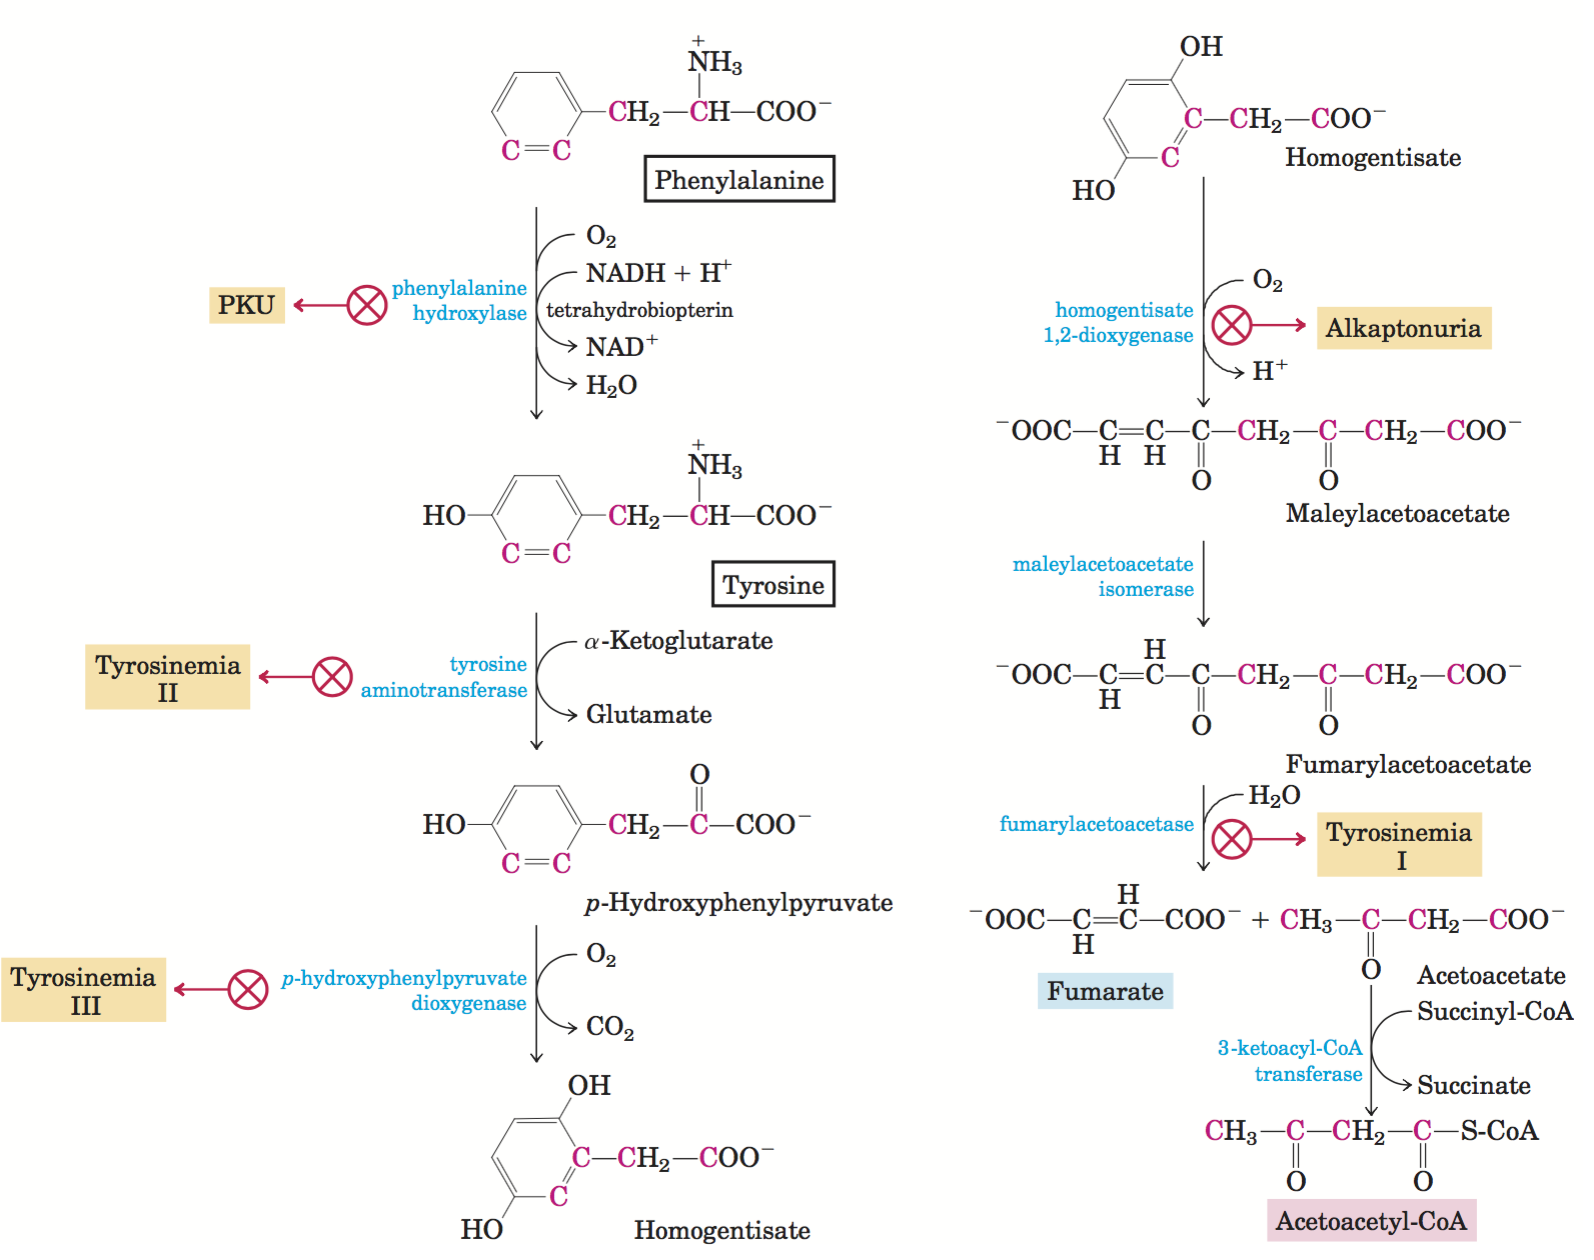
\includegraphics[width=\textwidth]{lehninger-IEMs}
\caption{Catabolic pathways for phenylalanine and tyrosine. In humans these amino acids are normally converted to acetoacetyl-CoA and fumarate. Genetic defects in many of these enzymes cause inheritable human diseases (shaded yellow).}
\label{fig:IEMs}
\end{figure}

Also see Figure \ref{fig:IEMs} from \cite{Lehninger_principlesBiochemistry} below for a pathway visualization of some more common IEMs.

\begin{quote}
Phenylketonuria can also be caused by a defect in the enzyme that catalyzes the regeneration of tetrahydrobiopterin. The treatment in this case is more complex than restricting the intake of phenylala- nine and tyrosine.

Tetrahydrobiopterin is also required for the formation of L-3,4 dihydroxyphenylalanine (L-dopa) and 5-hydroxytryptophan precursors of the neurotransmitters norepinephrine and serotonin, respectively and in phenylketonuria of this type, these pre- cursors must be supplied in the diet. Supplementing the diet with tetrahydrobiopterin itself is ineffective because it is unstable and does not cross the blood-brain barrier.
\end{quote}

\begin{figure}[h!]
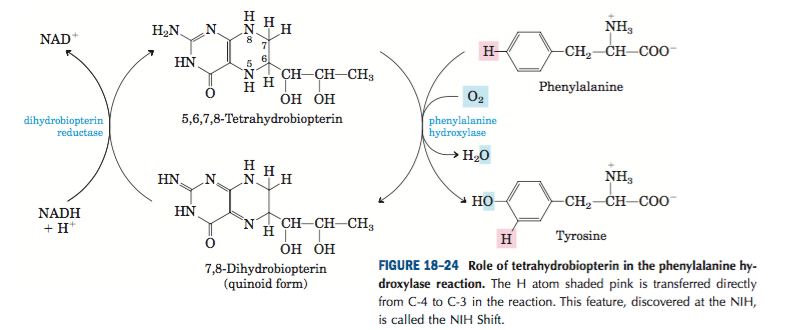
\includegraphics[width=\textwidth]{biopterin_salvage}
\caption{Role of tetrahydrobiopterin in the phenylalanine hydroxylase reaction.}
\label{fig:biopterin_salvage}
\end{figure}

Also see Figure \ref{fig:biopterin_salvage} from \cite{Lehninger_principlesBiochemistry} for the salvage reaction of biopterin.

\begin{tcolorbox}[width=\textwidth,colback={yellow},title={ASSIGNMENT},coltitle=white]

Go through tutorial 3: "3\_Phenylketonuria\_network\_illustration.ipynb".

This tutorial will introduce the reactions surrounding the hydroxylase and use flux map visualizations to make the results intuitive.

We will aim to show that the human metabolic reconstruction model is able to correctly predict that knockout of the PKU gene leads to problems in growth and neurotransmitter productions.

\end{tcolorbox}

\section{Biomarker prediction using flux variability a\-nalysis: intro}
Next we will focus on an intriguing application of the human metabolic model: the ability to predict the accumulation and depletion of any biomarker metabolites in extracellular tissues and fluids upon a specific mutation. 

The method we will utilize to do this is based on flux variability analysis and was presented originally in \cite{Shlomi2009}. It was subsequently used in the RECON2 paper to produce Figure 3.

\begin{tcolorbox}[width=\textwidth,colback={yellow},title={ASSIGNMENT},coltitle=white]

See \url{http://www.nature.com/nbt/journal/v31/n5/full/nbt.2488.html} and \url{http://www.ncbi.nlm.nih.gov/pmc/articles/PMC2683725/}. Read the abstract of the paper by Shlomi et al. Some essential parts of the method will be introduced in the notebooks below. 

Also take a look at the RECON2 paper again, specifically the part concerning Figure 3. Read the caption of the figure and the paragraph of text above it.
\end{tcolorbox}


\begin{tcolorbox}[width=\textwidth,colback={yellow},title={ASSIGNMENT},coltitle=white]

Go through tutorial 4: "4\_biomarker\_prediction\_Schlomi\_example.ipynb".

This notebook serves to illustrate in practice the method proposed by Shlomi et al.

\end{tcolorbox}


\section{Phenylketonuria: biomarker prediction}
Now that you have a feel for the method developed by Shlomi et al, we are going to apply it specifically to the PKU case. Note that this IEM was absent from Figure 3 in the RECON2 paper. It was however present in the article by Shlomi et al, but there the predecessor of RECON2, RECON1, was used for the prediction.

\begin{tcolorbox}[width=\textwidth,colback={yellow},title={ASSIGNMENT},coltitle=white]

Go through tutorial 5: "5\_biomarker\_prediction\_PKU.ipynb".

At the end of this tutorial you will have predicted biomarkers for both of the ways to get PKU: (1) mutating the hydroxylase and (2) mutating the salvation of the cofactor biopterin.

\end{tcolorbox}

\section{Concluding remarks}
We hope this tutorial achieved its aims to:
\begin{itemize}
\item Introduce you to programming with Python
\item Show you some real life examples of using metabolic maps and constraint-based modeling
\item Illustrate how genome-wide metabolic maps may be used to go beyond "textbook understanding" of pathways and show novel unexpected alternative ways to achieve metabolic tasks.
\item Highlighted one interesting way to use metabolic maps for biomarker prediction in tissues and biofluids.
\end{itemize}

For more information see the references below.

\bibliography{tutorial_citations}
\addcontentsline{toc}{section}{References}
\bibliographystyle{ieeetr}

\end{document}
